\pdfoutput=1
\documentclass[11pt]{article}
\usepackage[review]{naacl2021}
% Standard package includes
\usepackage{times}
\usepackage{latexsym}
\usepackage[T1]{fontenc}
\usepackage[utf8]{inputenc}
\usepackage{microtype}

% The preceding line is only needed to identify funding in the first footnote. If that is unneeded, please comment it out.
\usepackage{amsmath,amssymb,amsfonts}
\usepackage{algorithmic}
\usepackage{graphicx}
\usepackage{textcomp}
\usepackage{xcolor}

% \documentclass[a4paper, 11pt]{article}
% \usepackage[utf8]{inputenc}
% \usepackage{hyperref}
% \hypersetup{
%     colorlinks = true,
%     linkcolor = blue,
%     filecolor = magenta,      
%     urlcolor = cyan,
% }
\usepackage{multicol, float}
\usepackage{fancyhdr}
\usepackage{geometry}
\usepackage{graphicx, subfigure}
\usepackage[normalem]{ulem}
\useunder{\uline}{\ul}{}
\geometry{margin=1in}
\usepackage{subcaption}
% ------------------------------ Head

\title{\textbf{Transfer and Representation Learning with Memory Evaluation for Deep Reinforcement Learning}}
\author{
    \normalsize \textbf{Unique Divine (ud2127), Erik Skalnes (eas2301)} \\
    \normalsize Columbia University, Spring 2021 \\
}
\date{}

\begin{document}

\maketitle
\thispagestyle{fancy}
\lhead{IEOR 4540 - Data Mining Final Project}
\rhead{Spring 2021}
% \rfoot{Page \thepage}


\begin{abstract}
In this semester project, we experiment with transfer learning and deep reinforcement learning with raw image inputs in partially observable environments. To accomplish this task and allow full flexibility with the environment, we develop a new image-based, sparse-reward environment to iterate on new ideas. We make use of REINFORCE \cite{williams1992simple}, a Monte-Carlo policy gradient algorithm, for preliminary  training. In addition, we implement modules for the masked contrastive unsupervised representation learning algorithm, M-CURL \cite{zhu2020masked}, and experiment with enhancing our convolutional image encoder using an unsupervised auxiliary task. Additionally, we introduce some novel approaches for utilizing the context learned by Transformer modules to optimize the replay buffer and potentially further improve sample efficiency (Note, these experiments are still a work-in-progress). All code for our project, including the custom environment and all neural network systems, is available at \url{https://github.com/eskalnes/RL_memory/tree/main/rl_memory}.  
\end{abstract}

% ----------------------------------
\section{Introduction}
% ------------------------------

We are interested in developing RL agents that generalize well. Deep reinforcement learning (RL) as whole suffers from a sort of bottleneck, where even the most impressive breakthough systems of our time such as AlphaZero \cite{silver2017mastering}, Deep Q-Network \cite{mnih2015human}, and MuZero \cite{schrittwieser2020mastering} take upwards of a few hundred thousand or sometimes millions of episodes to converge to peak performance. The goal with this project is to use colored image inputs like the DQN paper for Atari except with greater sample efficiency and using lighter network modules. One of the main ways we do this is by learning predictive low-dimensional representations to speed up training. 

\subsection*{Transfer Learning Environment:}

For the purposes of our project, it was important to start out with a humble baseline for an environment that would still be relevant for the experiments we want to perform in both transfer learning and novel contributions to the processing of memories for RL optimization. Atari was too complex and many AI Gym environments in OpenAI are state-based and/or written in such a way that they are not easy to customize. So, we decided early on to implement a customizable environment that could allow both state (as in ``board game state'') and image-based training, multiple goals, multiple failure criteria, randomized starts, and even multiple agents. We came up with a simple, maze-like game (Fig. \ref{fig:custom-env}), where an agent tries to reach a goal for a positive reward without falling in a hole. 

\begin{figure}[H]
\centering
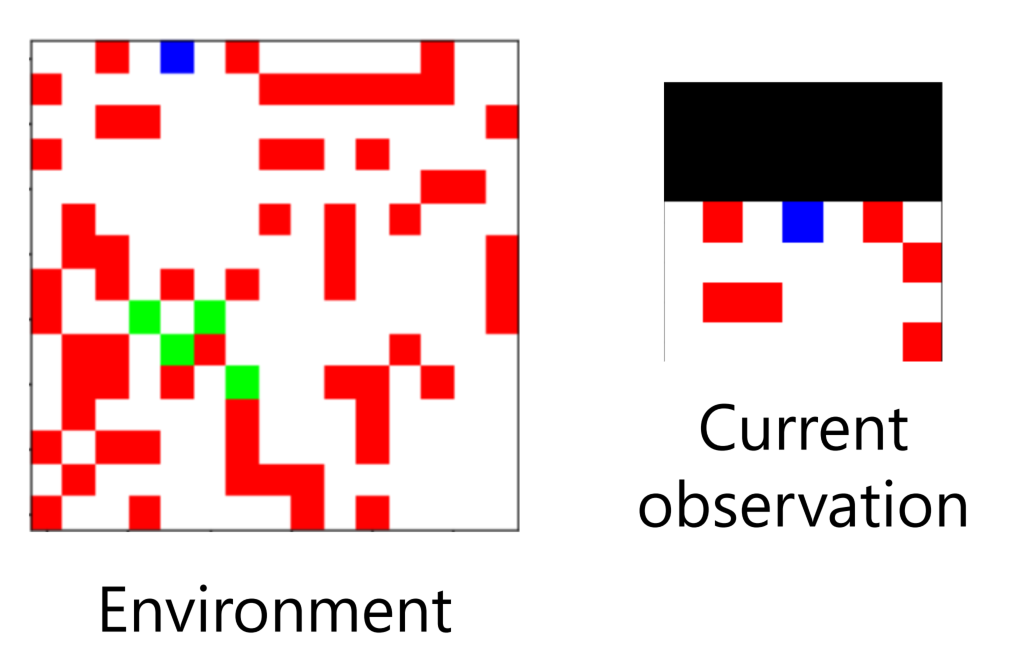
\includegraphics[width=0.99\linewidth]{figures/custom-env-background.png}
\caption{An example transfer learning environment. Here, the agent is the blue square and moves around in a 2-D space in any direction. If the agent steps in a hole (red), it dies, ending the episode, and producing a negative reward. If the agent reaches a goal (goal), it instead receives a positive reward.}
\label{fig:custom-env}
\end{figure}

This environment has undergone robust unit and integration testing so that it could be maximally useful as an open-sourced tool. It's available in our repo under \href{https://github.com/eskalnes/RL_memory/tree/main/rl_memory/custom_env}{\texttt{rl\_memory/custom\_env}} and functions with a similar API to that of the environments in \href{https://gym.openai.com/docs}{Open AI Gym}. 

\paragraph{Contrastive Learning: }
Contrastive learning is a self-supervised algorithm for representation learning developed in the computer vision community. It's an instance-level pre-training technique to get an encoder \cite{chen2020simple}, which here refers to a map from high-dimensional inputs (video, images, sound, etc.) to low-dimensional representations. Contrastive learning is particularly useful in the spare-reward setting because rewards often act as labels in deep reinforcement learning. Thus, self-supervised techniques that don't require labels can aid in improving sample efficiency\cite{laskin2020curl}. Self-supervised pre-training, just like word vectors, gives us a great starting point to vectorize an image into a semantically relevant geometric space. It's been a game changer in the computer vision world since around 2018  \cite{oord2018representation}.

\paragraph{Masked Training: }

In the Bidirectional Encoder Representations for Transformers \cite{devlin2018bert} paper, popularly known as ``BERT'', the authors found much success from the use of a masked language model. The basic idea was that some percentage of the input sequence is masked, and a transformer leverages its context in order to eventually predict the masked elements.     

\paragraph{Masked Contrastive Learning: }
Masked contrastive learning blends the idea of the masked language model with that of contrastive learning for training image encoders. With the M-CURL algorithm,  \cite{zhu2020masked} surpassed the current state of the art (CURL algorithm \cite{laskin2020curl} on many reinforcement learning tasks that use image inputs: 14 out of 16 environments from DMControl suite and 21 out of 26 environments from Atari 2600 Games. 




% ------------------------------
\section{What We Did: Methods \& Results}
% ------------------------------

Image based RL tasks are often framed as partially observable Markov decision processes (POMDPs), which can be described by the tuple $(\mathcal{O}, \mathcal{A}, p, r, \gamma)$, where 
\begin{itemize}
    \item $\mathcal{O}$ represents observations, a collection of images rendered from the environment, and 
    \item $\mathcal{A}$ is the action space,
\end{itemize}
Hence, $o_t \in \mathcal{O}$ represents the rendered image at time $t$ and $a_t\in \mathcal{A}$ denotes the action.

We can use observations $\{o_t\}$ as states for model-free RL on the simple environment (Fig. \ref{fig:custom-env}), i.e. $s_t = o_t$, however it is often useful to work with several video frames or stacks of images so that temporal information can be encapsulated in the state representation. Following the example of preprocessing in the DQN paper \cite{mnih2015human}, we also sometimes utilize a stack of $K$ ($>1$) consecutive observations as the input to capture more information. This sequence of observations makes a state, 
\[s_t = (o_{t-K+1}, o_{t-K+2}, \cdots, o_t).\] 
The collection of all states $\{s_t\}$ is denoted by $\mathcal{S}$. A convolutional netwok (ConvNet) encoder  $f_\theta$ with weights $\theta$ is used to map states $s_t\in \mathcal{S}$ into lower-dimensional representations. 

\subsection{Policy Gradient}
Our first experiment employs a paradigm similar to that of the first successful application of deep policy gradient algorithms for deep reinforcement learning in POMDPs, which to our knowledge was in the Minecraft control paper \cite{oh2016control}. 

We implement vanilla REINFORCE on a simple environment to show that it works. Then we pre-train a ConvNet encoded policy network with a simple environment in order to solve a much more difficult environment through transfer learning. We tried multiple configurations to no avail but eventually trained a performant agent with three changes:
\begin{enumerate}
    \item Small reward-shaping that punished an agent for staying still helped urge exploration and caused the agent to find more goals. 
    \item Holding the environment fixed each episode completely prevented the policy from understanding features that dealt with relative position, so the agent would inevitably converge to picking the same action each time. To fix this, we forced transfer learning by starting the agent on different environments each episode. 
    \item Over-saturating the reward signal didn't work with either extreme. If there were too many goals or too many holes, the agent would simply perform quasi-random actions. We found that a small 3 by 3 environment with one goal and one hole gave the fastest performance increase during training.  
\end{enumerate} 


\begin{figure*}[t]
\centering
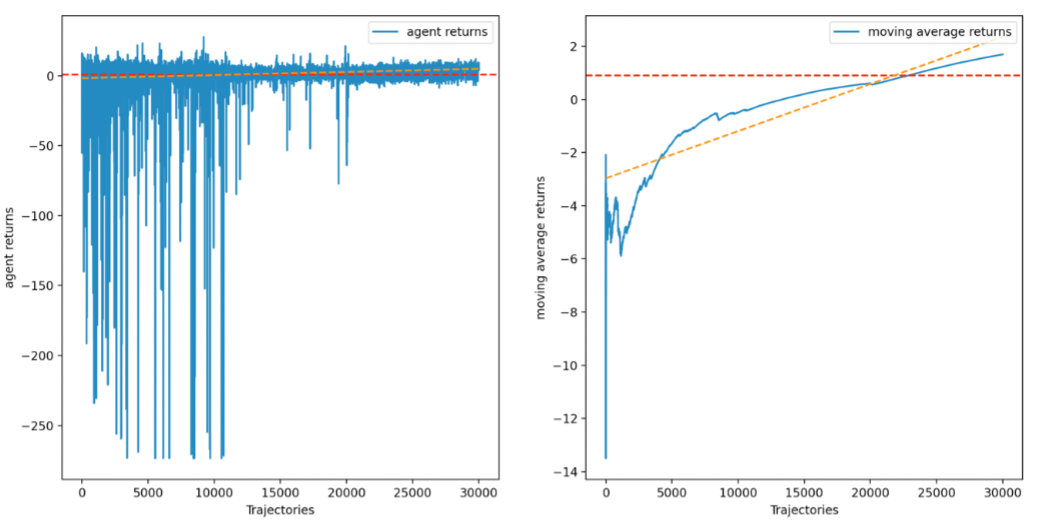
\includegraphics[width=0.99\linewidth]{figures/fig2-successful-agent.png}
\caption{Our agent succeeds to transfer learn onto new environment.}
\label{fig:custom-env}
\end{figure*}

The combination of these changes made an encoder and policy network that could succeed in more challenging, extreme environments. We show that the representation learned in the simple environment allows the agent to solve an environment (Fig. \ref{fig:custom-env}) that is effectively unsolvable with policy gradient methods after approximately 30,000 episodes of training on the 3 by 3 environment . Policy gradients fail in sparse reward environments, where the likelihood that an agent experiences a positive reward is so small that it converges to a policy that learns to avoid negative rewards instead, as described in \cite{kakade2002approximately}. We conclude that pre-training a representation is essential for improving sample efficiency in difficult environments. 

The point here is that a feature-rich representation of the agent state is essential to discovering good policies. To that end, we show that a policy gradient algorithm that uses a baseline that depends on having a good representation of state can solve problems even in the complicated domain of combinatorial optimization. We submit that this is a proof-of-concept for this type of memory-based algorithm in visual learning domains, where reinforcement learning algorithms will have to learn the representation, as one is not always readily available.  

\subsection{Masked Contrastive Learning}

For the purposes of further enhancing an image encoder without additional RL episodes, we implemented a similar style of framework to that used in Masked Contrastive Representation Learning for Reinforcement Learning \cite{zhu2020masked}. \textbf{Note}, a concise yet informative description of the method is included in the attached poster file. At the time of us writing this report, we're  trying to get the image encoder $f_\theta$ to learn from unsupervised pre-training on simulated episodes that are made (1) from random action sequences and (2) from previous trajectories saved from the policy gradient experiments. As it currently, stands, we have not benchmarked the effectiveness of masked contrastive learning, but this will continue in current/future work. 

% -----------------------------------------------
\section{Ongoing \& Future Work}
% -----------------------------------------------

We state some of our plans for the rest of the project because we intend to work to a publishable result. Since our training systems have managed to master this simple environment, we'll now test out other model-free algorithms in combination with the masked contrastive learning paradigm to see if we can increase sample efficiency even more. 

Additionally, we'll now benchmark on more challenging environments. It seems that the DMControl suite, robotic control tasks, and Atari games are the standard for testing image based RL systems, so these are options we're considering. There are two, key experiments we intend to conduct that have largely gone unexplored.

\begin{enumerate}
    \item Using the Transformer's sequence context to prioritize
sequences on the buffer.
    \item Use determinantal point processes to diversify the replay buffer and see if that improves training (credits to Professor Krzysztof Choromanski for this idea). 
\end{enumerate}

The poster that was submitted with this report has more details on the future experiments as well.

\newpage
\bibliography{bibliography} 
\bibliographystyle{acl_natbib}

% \appendix
% \section{Example Appendix}
% \label{sec:appendix}

% This is an appendix.

\end{document}




% \begin{center}
% \begin{tabular}{|c|c|c|c|}
% \hline
% \textbf{Batch size} & \textbf{Precision (bits)} 
%   & \textbf{Processes} & \textbf{Time (seconds/model)} \\ \cline{1-4}
% 1 & 32 & 1 & 43 \\
% 1 & 16 & 1 & 34 \\
% 1 & 32 & 4 & 20 \\
% 16 & 32 & 1 & 7 \\ 
% 16 & 16 & 2 & 4 \\ \hline 
% \end{tabular}
% \caption{caption.exe}
% \label{ablation}
% \end{center}
% \end{table*}begin{table*}[htbp]


% \begin{figure*}[]
% \subfigure[CPU Utilization in naive method]{ \includegraphics[width=0.5\linewidth]{figures/CPU_naive.png}}
% \subfigure[GPU Utilization in naive method]{ \includegraphics[width=0.5\linewidth]{figures/GPU_naive.png}}
% \subfigure[CPU Utilization in improved method]{ \includegraphics[width=0.5\linewidth]{figures/CPU_better.png}}
% \subfigure[GPU Utilization in improved method]{ \includegraphics[width=0.5\linewidth]{figures/GPU_better.png}}
% \label{fig:utilization}
% \caption{CPU and GPU utilization in base method vs. parallelized method. The base method has consistent GPU/CPU utilization through time. However, both CPU/GPU are under-utilized. In the improved method, we see significantly better CPU utilization. The spikes in the GPU correspond to the neural network training. The gaps in GPU utilization corresponds to time spent setting up the processes and models.}
% \end{figure*}